\begin{enumerate}
    %%%---1a---%%%
    \item Yes, $x_1^* = 1$, $x_2^* = 2$ is a feasible solution. The verification is done by substitution:
    \begin{align*}
     1 + 2 = 3& \geq 3,  &\checkmark  \\
     1 + 2 \cdot 2 = 5 & \leq 6,  &\checkmark  \\
     1 & \geq 1,  &\checkmark \\
     2 & \geq 1.  &\checkmark 
    \end{align*}
%
    The first and the third constraints are active at $(x_1^*,
    x_2^*)$. They are the two constraints that are verified with
    equality. The point lies at the intersection of the two lines that
    have $x_1 + x_2 = 3$ and $x_1 = 1$ as equations and is labeled
     $A$ in the figure below.
%
    %%%---1b---%%%
    \item Yes, $x_1^* = 2$, $x_2^* = 1.5$ is a feasible solution. The verification is done by substitution:
    \begin{align*}
     2 + 1.5 = 3.5 & \geq 3  &\checkmark \\
     2 + 2 \cdot 1.5 = 5 & \leq 6 & \checkmark  \\
     2 & \geq 1 & \checkmark  \\
     1.5 & \geq 1. & \checkmark  
    \end{align*}
%
    No constraint is active. Therefore, $(x_1^*, x_2^*)$ is an
    interior point. It is labeled $B$ in the figure below.

%
    %%%---1c---%%%
    \item The point $x_1^* = 1$, $x_2^* = 1$ is infeasible, as it
      violates the first constraint. 
    \begin{align*}
     1 + 1 = 2 & \not\geq 3 & \xmark   \\
     1 + 2 \cdot 1 = 3 & \leq 6 & \checkmark  \\
     1 & \geq 1 & \checkmark  \\
     1 & \geq 1. & \checkmark 
    \end{align*}
%    
    The point is labeled $C$ in the figure below.
\end{enumerate}

The graph below shows the feasible region for the problem.
     
     \begin{center}
     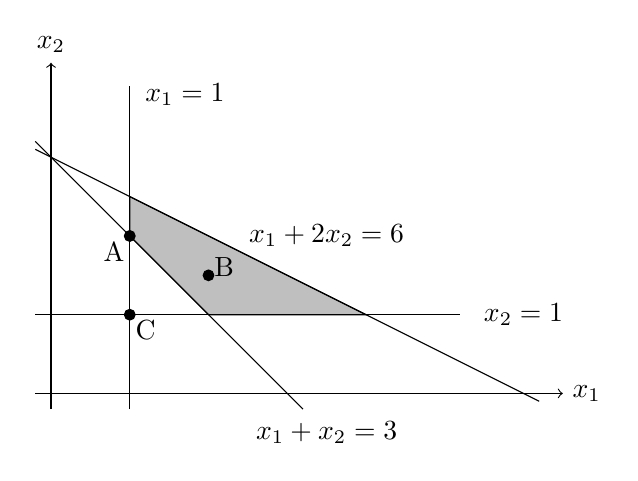
\begin{tikzpicture}[domain=-0.3:6.5,range=-0.5:4]
      
      \draw[fill=lightgray]  (1,2) -- (1,2.5) -- (4,1) -- (2,1) -- cycle;
      \draw[->] (-0.2,0) -- (6.5,0) node[right] {$x_1$};
      \draw[->] (0,-0.2) -- (0,4.2) node[above] {$x_2$};
      
      \draw[color=black] (-0.2,1) -- (5.2,1);
      	\node at (6,1) {$x_2 = 1$};
      
      \draw[color=black] (1,-0.2) -- (1,3.9);
      	\node at (1.7,3.8) {$x_1 = 1$};
      
      \draw[color=black] (-0.2,3.2) -- (3.2,-0.2);
      \node at (3.5,-0.5) {$x_1 + x_2 = 3$};
      
      \draw[color=black] (-0.2,3.1) -- (6.2,-0.1);
      \node at (3.5,2) {$x_1 + 2 x_2 = 6$};
      
%      \draw[pattern=vertical lines]  (1,2) -- (1,2.5) -- (4,1) -- (2,1) -- cycle;
      
      \node [circle,fill=black,draw,scale=0.2] at (1,2) {A};
      \node at (0.8,1.8) {A};
      \node [circle,fill=black,draw,scale=0.2] at (2,1.5) {B};
      \node at (2.2,1.6) {B};
      \node [circle,fill=black,draw,scale=0.2] at (1,1) {C};
      \node at (1.2,0.8) {C};
    
    \end{tikzpicture}
    \end{center}

